%!TEX root = main.tex

\section{The Method of Steepest Descent}

The method of Steepest Descent is based upon the following property of gradients that we learned in Vector Calculus:

\begin{theorem}
If $f \colon \field{R}^d \to \field{R}$ is continuously differentiable, then at any point $\x \in \field{R}^d$, the vector $-\gradient{f}(\x)$ points in the direction of most rapid decrease for $f$ at $\x$.  The rate of decrease of $f$ at $\x$ in this direction is precisely $-\norm{\gradient{f}(\x)}$.
\end{theorem}

\begin{remark}\index{Steepest descent!direction of}
For this reason, the vector $-\gradient{f}(\x)$ is called the \emph{direction of steepest descent} of $f$ at $\x$.
\end{remark}

\separator

In order to search for a local minimum for a twice continuously differentiable function $f\colon \field{R}^d \to \field{R}$, we start by choosing an initial guess $\x_0$.  
\begin{enumerate}
	\item Restrict the function $f$ over the line through $\x_0$ in the direction of $-\gradient{f}(\x_0)$:
	\begin{equation*}
	\varphi_0(t) = f\big( \x_0 - t \gradient{f}(\x_0) \big), \quad t\geq 0
	\end{equation*}
	\item Search for the value of $t_0 \geq 0$ that minimizes $\varphi_0$, and set 
	\begin{equation*}
	\x_1 = \x_0 - t_0\gradient{f}(\x_0)
	\end{equation*}
	\item Repeat this process to get the sequence
	\begin{gather}\label{equation:SteepestDescent}
	\begin{split}
	&\x_{n+1} = \x_n - t_n \gradient{f}(\x_n), \\ &t_n = \argmin_{t\geq 0} \varphi_n(t) = \argmin_{t\geq 0} f\big(\x_n - t\gradient{f}(\x_n)\big)
	\end{split}
	\end{gather}
\end{enumerate}

\begin{remark}\index{Steepest descent!sequence of}
Sequences constructed following the formula in \eqref{equation:SteepestDescent} are said to be \emph{sequences of Steepest Descent} for $f$.

Unlike Newton's method, this algorithm guarantees that these sequences are non-increasing: $f(\x_{n+1}) \leq f(\x_n)$ for all $n \in \field{N}$.  And even better: if there is convergence, their limit must a critical point of $f$.  These results are formalized in Theorems \ref{theorem:SteepestDescentDescends} and \ref{theorem:SteepestDescentConvergesToCritical}  below.

Steepest descent sequences have another interesting property: on each step $n$, the direction of descent $x_{n+1} - x_n$ is perpendicular to the direction of the next step!  We state and prove this result in Theorem \ref{theorem:SteepestDescentPerpSteps}.
\end{remark}

\begin{theorem}\label{theorem:SteepestDescentDescends}
Let $f\colon \field{R}^d \to \field{R}$ be a continuously differentiable real-valued function, and let $\{ \x_n \}_{n\in\field{N}}$ be a sequence of steepest descent for $f$.  If $\gradient{f}(\x_N) \neq 0$, then $f(\x_{N+1}) < f(\x_N)$.
\end{theorem}

\begin{theorem}\label{theorem:SteepestDescentConvergesToCritical}
Let $f\colon \field{R}^d \to \field{R}$ be a real-valued function, let $\x_0 \in \field{R}^d$ be an initial guess.  Assume $S = \{ \x \in \field{R}^d :  f(\x) \leq f(\x_0) \}$ is a compact set and $f$ is continuously differentiable in $S$.  Under these conditions, the limit of any convergent subsequence of the associated sequence of steepest descent $\{ \x_n \}_{n\in \field{N}}$ is a critical point of $f$.
\end{theorem}

\begin{theorem}\label{theorem:SteepestDescentPerpSteps}
Let $f \colon \field{R}^d \to \field{R}$ be a continuously differentiable real-valued function, and $\{ \x_n \}_{n\in\field{N}}$ a sequence of steepest descent for $f$.  For any $n \in \field{N}$, $\langle \x_{n+2} - \x_{n+1}, \x_{n+1} - \x_n \rangle = 0$.
\end{theorem}
\begin{proof}
Consider for each $n \in \field{N}$ the function $\varphi_n(t) = f\big(\x_n -t \gradient{f}(\x_x)\big)$, with a global minimum at $t_n \geq 0$.  It must then be
\begin{equation*}
0 = \varphi_n'(t_n) = \langle \gradient{f}(\x_n), -\gradient{f}\big( \x_n - t_n \gradient{f}(\x_n)\big) \rangle = - \langle \gradient{f}(\x_{n+1}), \gradient{f}(\x_n) \rangle,
\end{equation*}
which proves that the gradient of consecutive terms of the sequence of steepest descent for $f$ are perpendicular.  Now, by virtue of the recurrence formula \eqref{equation:SteepestDescent},
\begin{align*}
\langle \x_{n+2} - \x_{n+1}, &\x_{n+1} - \x_n \rangle = \langle t_{n+1}\gradient{f}(\x_{n+1}), t_n \gradient{f}(\x_n) \rangle \\
&= t_{n+1}t_n \langle \gradient{f}(\x_{n+1}), \gradient{f}(\x_n) \rangle = 0, 
\end{align*}
which proves the statement.
\end{proof}

\begin{example}
For the polynomial function $p_4(x,y) = x^4-4xy+y^4$ from Example \ref{example:NewtonPoly4}, using the same initial guesses as in Example \ref{example:preNewton4poly4}, we find the following behavior:
\begin{itemize}
	\item Starting at $(x_0, y_0) = (-1.0,1.0)$, the sequence also converges to $(0,0)$, but this time in one step.
	% \begin{table}[ht!]
	\begin{center}
	\begin{tabular}{|r|r|r|r|} \hline 
	$n$ & $x_n$ & $y_n$ & $f(x_n,y_n)$ \\ \hline \hline 
	$0$ & $-1.000000$ & $1.000000$ & $6.000000$ \\ \hline 
	$1$ & $0.000000$ & $0.000000$ & $0.000000$ \\ \hline 
	$2$ & \texttt{nan} & \texttt{nan} & \texttt{nan} \\ \hline 
	\end{tabular}
	% \caption{Steepest Descent: Convergence to $(0,0)$ accurately in exactly one step.}
	% \label{table:SD00}
	% \end{table}
	\end{center}
	\item Starting at $(x_0,y_0) = (3.5, 2.1)$, the sequence converges to $(1,1)$.
	% \begin{table}[ht!]
	\begin{center}
	\begin{tabular}{|r|r|r|r|} \hline 
	$n$ & $x_n$ & $y_n$ & $f(x_n,y_n)$ \\ \hline \hline 
	$0$ & $3.500000$ & $2.100000$ & $140.110600$ \\ \hline 
	$1$ & $1.044472$ & $1.753064$ & $3.310777$ \\ \hline 
	$2$ & $1.141931$ & $1.063276$ & $-1.878163$ \\ \hline 
	$3$ & $1.008581$ & $1.044435$ & $-1.988879$ \\ \hline 
	$4$ & $1.013966$ & $1.006319$ & $-1.998931$ \\ \hline 
	$5$ & $1.000898$ & $1.004472$ & $-1.999891$ \\ \hline 
	$6$ & $1.001437$ & $1.000651$ & $-1.999989$ \\ \hline 
	$7$ & $1.000093$ & $1.000461$ & $-1.999999$ \\ \hline 
	\end{tabular}~\begin{tabular}{|r|r|r|r|} \hline 
	$n$ & $x_n$ & $y_n$ & $f(x_n,y_n)$ \\ \hline \hline 
	$8$ & $1.000149$ & $1.000067$ & $-2.000000$ \\ \hline 
	$9$ & $1.000010$ & $1.000048$ & $-2.000000$ \\ \hline 
	$10$ & $1.000015$ & $1.000007$ & $-2.000000$ \\ \hline 
	$11$ & $1.000001$ & $1.000005$ & $-2.000000$ \\ \hline 
	$12$ & $1.000002$ & $1.000001$ & $-2.000000$ \\ \hline 
	$13$ & $1.000000$ & $1.000001$ & $-2.000000$ \\ \hline 
	$14$ & $1.000000$ & $1.000000$ & $-2.000000$ \\ \hline 
	$15$ & $1.000000$ & $1.000000$ & $-2.000000$ \\ \hline 
	\end{tabular}
	% \caption{Steepest Descent: Convergence to $(1,1)$ with 6-digit accuracy in 13 steps.}
	% \label{table:SD11}
	% \end{table}
	\end{center}
	\item Starting at $(x_0, y_0) = (-13.5, -7.3)$, the sequence converges to $(1,1)$ as well.
	% \begin{table}[ht!]
	\begin{center}
	\begin{tabular}{|r|r|r|r|} \hline 
	$n$ & $x_n$ & $y_n$ & $f(x_n,y_n)$ \\ \hline \hline 
	$0$ & $-13.500000$ & $-7.300000$ & $35660.686600$ \\ \hline 
	$1$ & $2.362722$ & $-4.871733$ & $640.498302$ \\ \hline 
	$2$ & $1.434154$ & $1.194162$ & $-0.586492$ \\ \hline 
	$3$ & $1.021502$ & $1.130993$ & $-1.896212$ \\ \hline 
	$4$ & $1.038817$ & $1.017881$ & $-1.991558$ \\ \hline 
	$5$ & $1.002305$ & $1.012291$ & $-1.999167$ \\ \hline 
	$6$ & $1.003909$ & $1.001808$ & $-1.999917$ \\ \hline 
	$7$ & $1.000236$ & $1.001246$ & $-1.999992$ \\ \hline 
	\end{tabular}~\begin{tabular}{|r|r|r|r|} \hline 
	$n$ & $x_n$ & $y_n$ & $f(x_n,y_n)$ \\ \hline \hline 
	$8$ & $1.000399$ & $1.000185$ & $-1.999999$ \\ \hline 
	$9$ & $1.000024$ & $1.000127$ & $-2.000000$ \\ \hline 
	$10$ & $1.000041$ & $1.000019$ & $-2.000000$ \\ \hline 
	$11$ & $1.000002$ & $1.000013$ & $-2.000000$ \\ \hline 
	$12$ & $1.000004$ & $1.000002$ & $-2.000000$ \\ \hline 
	$13$ & $1.000000$ & $1.000001$ & $-2.000000$ \\ \hline 
	$14$ & $1.000000$ & $1.000000$ & $-2.000000$ \\ \hline 
	$15$ & $1.000000$ & $1.000000$ & $-2.000000$ \\ \hline 
	\end{tabular}
	% \caption{Steepest Descent: Convergence to $(1,1)$ with 6-digit accuracy in 14 steps.}
	% \label{table:SD-1-1}
	% \end{table}
	\end{center}
\end{itemize}
\end{example}

\begin{example}\label{example:SDR}\index{Function!Rosenbrock}
Notice what happens when we try to implement the same process on the Rosenbrock function $\mathcal{R}_{1,1}(x,y) = (1-x)^2 + (y-x^2)^2$, with the initial guess $(x_0, y_0) = (-2,2)$.  The sequence does converge to the minimum $(1,1)$, albeit very slowly.
\begin{center}
\begin{tabular}{|r|r|r|r|} \hline 
 $n$ & $x_n$ & $y_n$ & $f(x_n,y_n)$ \\ \hline \hline 
$0$ & $-2.000000$ & $2.000000$ & $13.000000$ \\ \hline 
$1$ & $-0.166290$ & $2.309522$ & $6.567163$ \\ \hline 
$2$ & $0.256054$ & $-0.056128$ & $0.568264$ \\ \hline 
$3$ & $0.613477$ & $0.007683$ & $0.285318$ \\ \hline 
$4$ & $0.568566$ & $0.259241$ & $0.190235$ \\ \hline 
$5$ & $0.715784$ & $0.285524$ & $0.132227$ \\ \hline 
$6$ & $0.689755$ & $0.431319$ & $0.098227$ \\ \hline 
$7$ & $0.779264$ & $0.447299$ & $0.074310$ \\ \hline 
$8$ & $0.761554$ & $0.546496$ & $0.057977$ \\ \hline 
$9$ & $0.823325$ & $0.557524$ & $0.045696$ \\ \hline 
$10$ & $0.810322$ & $0.630358$ & $0.036667$ \\ \hline 
$11$ & $0.855862$ & $0.638488$ & $0.029614$ \\ \hline 
$12$ & $0.845883$ & $0.694385$ & $0.024199$ \\ \hline 
$13$ & $0.880846$ & $0.700627$ & $0.019862$ \\ \hline 
$14$ & $0.872964$ & $0.744776$ & $0.016437$ \\ \hline 
$15$ & $0.900551$ & $0.749702$ & $0.013647$ \\ \hline 
$16$ & $0.894200$ & $0.785276$ & $0.011399$ \\ \hline 
\end{tabular}~\begin{tabular}{|r|r|r|r|} \hline
 $n$ & $x_n$ & $y_n$ & $f(x_n,y_n)$ \\ \hline \hline 
$17$ & $0.916394$ & $0.789239$ & $0.009544$ \\ \hline 
$18$ & $0.911201$ & $0.818326$ & $0.008028$ \\ \hline 
$19$ & $0.929317$ & $0.821560$ & $0.006766$ \\ \hline 
$20$ & $0.925024$ & $0.845608$ & $0.005723$ \\ \hline 
$21$ & $0.939976$ & $0.848277$ & $0.004847$ \\ \hline 
$22$ & $0.936397$ & $0.868329$ & $0.004118$ \\ \hline 
$23$ & $0.948845$ & $0.870551$ & $0.003502$ \\ \hline 
$24$ & $0.945840$ & $0.887385$ & $0.002986$ \\ \hline 
$25$ & $0.956276$ & $0.889248$ & $0.002548$ \\ \hline 
$26$ & $0.953739$ & $0.903457$ & $0.002178$ \\ \hline 
$27$ & $0.962537$ & $0.905028$ & $0.001864$ \\ \hline 
$28$ & $0.960386$ & $0.917075$ & $0.001597$ \\ \hline 
$29$ & $0.967837$ & $0.918405$ & $0.001369$ \\ \hline 
$30$ & $0.966007$ & $0.928657$ & $0.001176$ \\ \hline 
$31$ & $0.972342$ & $0.929788$ & $0.001010$ \\ \hline 
$32$ & $0.970780$ & $0.938539$ & $0.000869$ \\ \hline 
$33$ & $0.976182$ & $0.939503$ & $0.000748$ \\ \hline 
\end{tabular}
\end{center}
\end{example}

\begin{figure}[ht!]
\begin{tabular}{c}
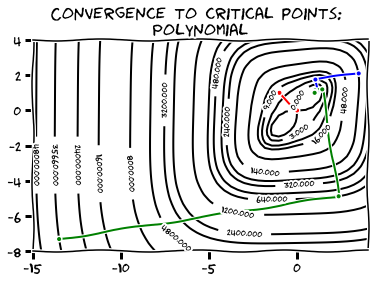
\includegraphics[width=0.65\linewidth]{images/convergenceSteepest.png} \\
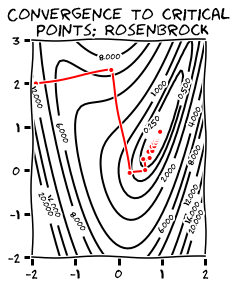
\includegraphics[width=0.65\linewidth]{images/SDR3.png}
\end{tabular}
\caption{The Method of Steepest Descent}
\label{figure:SteepestConvergence}
\end{figure}

\subsection{Efficiency of Steepest Descent Method}

The analysis of efficiency of the method of Steepest descent is quite involved, but it boils down to studying the efficiency of Steepest descent for quadratic functions---since any function can be approximated using a Taylor's polynomial of degree two.  We will study that easier case in these notes.

\begin{theorem}[Taylor's Formula]
If $f\colon \field{R}^d \to \field{R}$ is a real-valued function of $d$ variables with continuous first and second partial derivatives on $\field{R}^d$, then for any choice $\x, \y \in \field{R}^d$, there exists a point $\boldsymbol{\xi} = \boldsymbol{\xi}(\x, \y)$ in the segment joining $\x$ and $\y$ so that
\begin{equation*}
f(\x) = f(\y) + \langle \gradient{f}(\y), \x - \y \rangle + \tfrac{1}{2} \quadratic{\Hess{f}(\boldsymbol{\xi})}(\x - \y)
\end{equation*}
\end{theorem}

\separator

Assume we have a quadratic function $p\colon \field{R}^d \to \field{R}$ satisfying $p(\boldsymbol{0}) = 0$.  There exist a $d$-dimensional vector $D = \big[q_1, \dotsc, q_d\big]$ and a symmetric matrix $Q = \big[ q_{jk} \big]_{j,k=1}^d$ (with $q_{jk}=q_{kj}$ for all $1\leq j,k \leq d$) so that
\begin{equation*}
p(\x) = \langle D, \x \rangle + \tfrac{1}{2}\quadratic{Q}(\x) = \sum_{k=1}^d \big( \tfrac{1}{2}q_{kk}x_k^2 + q_k x_k\big) + \sum_{1\leq j<k \leq d} q_{jk} x_j x_k
\end{equation*}
The gradient of this function is thus $\gradient{p}(\x) = x \cdot Q + D$.  It has one unique critical point $\xstar = -D Q^{-1}$ (Why?).  At that point, it is 
\begin{align}
p(\xstar) &= \tfrac{1}{2} \big( -D Q^{-1} \big)  Q \transpose{\big( -D Q^{-1} \big)} + D \transpose{\big( -D Q^{-1} \big)} \nonumber \\ 
&= \tfrac{1}{2} D Q^{-1} \transpose{D} - D Q^{-1} \transpose{D} \nonumber \\
&= -\tfrac{1}{2} D Q^{-1} \transpose{D} = -\tfrac{1}{2}\quadratic{(Q^{-1})}(D). \label{equation:pstarSD}
\end{align}
If $\x_n$ is a term in a sequence of steepest descent, then to compute $\x_{n+1}$ we proceed as follows:
\begin{enumerate}
	\item The direction of steepest descent at $\x_n$ is 
	\begin{equation*}\v_n = -\gradient{p}(\x_n) = -(x_n Q + D).
	\end{equation*}
	\item The restriction $\varphi\colon (0,\infty) \to \field{R}$ of the quadratic function $p$ over the half-line through $\x_n$ in the direction $\v_n$ is given by
	\begin{align*}
	\varphi(t) &= p( \x_n + t \v_n ) \\
	&= \tfrac{1}{2}(\x_n + t\v_n ) Q \transpose{(\x_n + t\v_n )} + D\transpose{(\x_n + t\v_n )} \\
	&= \tfrac{1}{2} \x_n Q \transpose{(\x_n + t\v_n )} + \tfrac{1}{2}t\v_n Q \transpose{(\x_n + t\v_n )} \\
	&\quad+D \transpose{\x}_n + tD \transpose{\v}_n \\
	&= \tfrac{1}{2}\x_n Q \transpose{\x}_n + \tfrac{1}{2} t\x_n Q \transpose{\v}_n + \tfrac{1}{2} t \v_n Q \transpose{\x}_n + \tfrac{1}{2} t^2 \v_n Q \transpose{\v}_n \\
	&\quad + D \transpose{\x}_n + t D \transpose{\v}_n \\
	&= \tfrac{1}{2} \underbrace{\v_n Q \transpose{\v}_n}_{\quadratic{Q}(\v_n)} t^2 + \underbrace{\tfrac{1}{2}\x_n Q \transpose{\x}_n + D \transpose{\x}_n}_{p(\x_n)} + tD\transpose{\v}_n + t \x_n Q \transpose{\v}_n \\
	&= \tfrac{1}{2} \quadratic{Q}(\v_n) t^2  + p(\x_n) + t \underbrace{\big( x_n Q + D \big)}_{-\v_n} \transpose{\v}_n \\
	&= \tfrac{1}{2}t^2 \v_n Q \transpose{\v}_n -  t \v_n \transpose{\v}_n + p(\x_n) \\
	&= \tfrac{1}{2} \quadratic{Q}(\v_n)t^2 - \norm{\v_n}^2 t + p(\x_n)
	\end{align*}
	\item The restriction function has its global minimum at
	\begin{equation*}
	t_n = \frac{\norm{\v_n}^2}{\quadratic{Q}(\v_n)};
	\end{equation*}
	therefore, the next iteration occurs at
	\begin{equation*}
	x_{n+1} = x_n + t_n \v_n = x_n + \frac{\norm{\v_n}^2}{\quadratic{Q}(\v_n)} \v_n 
	\end{equation*}
\end{enumerate}

\separator

We want to observe the convergence behavior of the sequence of evaluations $\{ p(\x_n) \}_{n \in \field{N}}$ to $p(\xstar)$.  We have
\begin{align*}
p(\x_{n+1}) &= p(\x_n + \tfrac{\norm{\v_n}^2}{\quadratic{Q}(\v_n)} \v_n) \\
&= \tfrac{1}{2} \quadratic{Q}(\v_n) \big( \tfrac{\norm{\v_n}^2}{\quadratic{Q}(\v_n)} \big)^2 - \norm{\v_n}^2 \tfrac{\norm{\v_n}^2}{\quadratic{Q}(\v_n)} + p(\x_n) \\
&= p(\x_n) - \frac{\norm{\v_n}^4}{2\quadratic{Q}(\v_n)}; 
\intertext{therefore,}
\frac{p(\x_{n+1}) - p(\xstar)}{p(\x_n)- p(\xstar)} &= \frac{p(\x_n) - p(\xstar) - \frac{\norm{\v_n}^4}{2\quadratic{Q}(\v_n)}}{p(\x_n) - p(\xstar)} \\
&= 1 - \frac{\norm{\v_n}^4}{ 2\quadratic{Q}(\v_n) \big( p(\x_n) - p(\xstar) \big)} \\
&= 1 - \frac{\norm{\v_n}^4}{2\quadratic{Q}(\v_n) \big( \tfrac{1}{2}\x_n Q \transpose{\x}_n + D \transpose{\x}_n + \tfrac{1}{2} DQ^{-1}\transpose{D} \big)} \\
&= 1 - \frac{\norm{\v_n}^4}{ \quadratic{Q}(\v_n) \big( \x_n Q \transpose{\x}_n+ 2D\transpose{\x}_n + DQ^{-1}\transpose{D} \big) }.
\end{align*}
Note in the denominator we may rewrite some of the terms:
\begin{align*}
\x_n Q \transpose{\x}_n &= \x_n Q (Q^{-1}Q) \transpose{\x}_n = (\x_n Q) Q^{-1} \transpose{(\x_n Q)}, \\
2D \transpose{\x}_n &= D\transpose{\x}_n + D\transpose{\x}_n = \x_n \transpose{D} + D (Q^{-1}Q) \transpose{\x}_n \\
&= \x_n (QQ^{-1}) \transpose{D} + D Q^{-1} \transpose{(\x_n Q)} \\
&= (\x_n Q) Q^{-1} \transpose{D} + D Q^{-1} \transpose{(\x_n Q)}.
\end{align*} 
This allows us to rewrite in the following convenient form 
\begin{align*}
\frac{p(\x_{n+1}) - p(\xstar)}{p(\x_n)- p(\xstar)} &= 1 - \frac{\norm{\v_n}^4}{ \quadratic{Q}(\v_n) (\x_n Q + D) Q^{-1} \transpose{(\x_nQ + D)} } \\
&= 1 - \frac{\norm{\v_n}^4}{\quadratic{Q}(\v_n) \quadratic{(Q^{-1})}(\v_n)}.
\end{align*}

We are ready to state the main result of this subsection:
\begin{theorem}\label{theorem:KantorovichEstimate}
Given a $d$-dimensional vector $D$, and a positive definite symmetric matrix $Q$ of size $d \times d$, consider the quadratic function $p(\x) = \tfrac{1}{2}\quadratic{Q}(\x) + \langle D , \x \rangle$.  Any sequence $\{ \x_n \}_{n \in \field{N}}$ of steepest descent converges to the global minimum $\xstar = -DQ^{-1}$.  The sequence of evaluations $\{ p(\x_n) \}_{n \in \field{N}}$ converges linearly to $p(\xstar) = -\tfrac{1}{2}\quadratic{(Q^{-1})}(D)$.  In particular, if $0 < \lambda_1 \leq \lambda_2 \leq \dotsb \leq \lambda_d$ are the eigenvalues of $Q$, then 
\begin{equation*}
\frac{p(\x_{n+1}) - p(\xstar)}{p(\x_n)- p(\xstar)} \leq \bigg( \frac{\lambda_d -\lambda_1}{\lambda_d + \lambda_1} \bigg)^2
\end{equation*}
\end{theorem}
\begin{proof}
We start by offering the following lower bound estimate\footnote{This is left as and advanced exercise. It is not too tricky; if you are stuck, see e.g.~\cite[section 1.3.1]{bertsekas1999nonlinear} for a proof.} involving the associated directions of steepest descent $\v_n$ in terms of the largest and smallest eigenvalues of $Q$.  For all $n \in \field{N}$,
\begin{equation}\label{equation:KantorovichEstimate}
\frac{\norm{\v_n}^4}{\quadratic{Q}(\v_n) \quadratic{(Q^{-1})}(\v_n)} \geq \frac{4\lambda_0\lambda_d}{(\lambda_0 + \lambda_d)^2}
\end{equation}
We have then
\begin{align*}
\frac{p(\x_{n+1}) - p(\xstar)}{p(\x_n)- p(\xstar)} &= 1 - \frac{\norm{\v_n}^4}{ \quadratic{Q}(\v_n) \quadratic{(Q^{-1})}(\v_n) } \\
&\leq 1 - \frac{4\lambda_1 \lambda_d}{(\lambda_1 + \lambda_d)^2} = \bigg( \frac{\lambda_d - \lambda_1}{\lambda_d + \lambda_1} \bigg)^2 \qedhere
\end{align*}
\end{proof}

\begin{example}\label{example:SDconvergenceRate}
The global minimum value of the quadratic function $p(x,y) = 5x^2 + 5y^2 -xy -11x +11y +11$ is zero, and found at $(1,-1)$.  Notice that we may write this function in the form $p(x,y) = \tfrac{1}{2}\quadratic{Q}(x,y) + \langle D, [x,y] \rangle + 11$, where
\begin{align*}
D &= [ -11, 11], \\
Q &= \begin{bmatrix} 10 & -1 \\ 10 & -1 \end{bmatrix}.
\end{align*}
The symmetric matrix $Q$ has eigenvalues $\lambda_1 = 9 >0$, $\lambda_2 = 11 > 0$ and is therefore positive definite.  Theorem \ref{theorem:KantorovichEstimate} states that sequences of steepest descent exhibit linear convergence with a rate of convergence not larger than $\delta = \big( \tfrac{11-9}{11+9} \big)^2 = 0.01$.

Observe the computations of the first six iterations for values of the ratios $\frac{p(\x_n)}{p(\x_{n-1})}$ when we use $(1.5,3.5)$ as our initial guess.
\begin{center}
\begin{tabular}{|r|r|r|r|r|} \hline 
 $n$ & $x_n$ & $y_n$ & $p(x_n,y_n)$ & $\boldsymbol{\frac{p(x_n,y_n)}{p(x_{n-1},y_{n-1})}}$ \\ \hline \hline 
$0$ & $1.5000000000$ & $3.5000000000$ & $100.2500000000$ &  \\ \hline 
$1$ & $1.4498874016$ & $-0.9600212545$ & $1.0019989373$ & $\boldsymbol{0.0099950019}$ \\ \hline 
$2$ & $1.0049975009$ & $-0.9550224916$ & $0.0100149812$ & $\boldsymbol{0.0099950019}$ \\ \hline 
$3$ & $1.0044966254$ & $-0.9996004124$ & $0.0001000998$ & $\boldsymbol{0.0099950019}$ \\ \hline 
$4$ & $1.0000499500$ & $-0.9995504497$ & $0.0000010005$ & $\boldsymbol{0.0099950019}$ \\ \hline 
$5$ & $1.0000449438$ & $-0.9999960061$ & $0.0000000100$ & $\boldsymbol{0.0099950042}$ \\ \hline 
$6$ & $1.0000004993$ & $-0.9999955067$ & $0.0000000001$ & $\boldsymbol{0.0099950528}$ \\ \hline 
\end{tabular}
\end{center}
\end{example}
